
\subsection{Motivación}

\begin{frame}
		\frametitle{Motivación}
		Es usual encontrar contextos de aplicación en los cuales la ubicación geográfica de los datos a representar adquiere una importancia fundamental a la hora de recuperarlos. \pause \\
		Tan es asi que se han desarrollado sistemas de administradores de bases de datos específicamente orientados a manejar eficientemente estos datos. \pause \\
		Algunos ejemplos tangibles de tales sistemas son:
		\begin{itemize}
				\item	Servicios web (encontrar el servidor más cercano al cliente) \pause
				\item	Astronomía (encontrar todas las estrellas cercanas a un punto) \pause
				\item	Compañía de seguros (qué casas están más expuestas a desastres naturales?) \pause
				\item	Control de aerolínas (dónde está cada avión?)
		\end{itemize}
\end{frame}

\begin{frame}
		\frametitle{Definición de DB espacial}
		Una base de datos espacial es una DB que provee soporte interno para manejar eficientemente datos espaciales. \pause
		La mayoría permite representar objetos geométricos como puntos, lineas y polígonos; pero algunas además se extienden a estructuras más complejas como objetos tridimensionales. \pause
		Implementan un indexado espacial, más eficiente que el indexado tradicional para estos dominios de aplicación; algoritmos optimizados para procesar operaciones espaciales, y reglas para agilizar las consultas. \pause
		Además, proveen tipos de datos abstractos espaciales y un lenguaje de consultas desde las cuales pueden ser manipulados.
\end{frame}

\begin{frame}
		\frametitle{Índices espaciales}
		Los índices espaciales se utilizan en las bases de datos de este tipo para reducir los tiempos de búsqueda. \pause
		Aunque existen varias implementaciones de índices espaciales, el método preferido se conoce como {\bf árbol-R}, una estructura de datos en forma de árbol de búsqueda balanceado, en donde los objetos cercanos se agrupan en su rectángulo delimitador mínimo (minimum bounding rectangle), ubicado un nivel más alto que ellos (la "R" en el nombre del índice es por "rectángulo"). \pause
		En las hojas se encuentran los objetos de nuestra base de datos. \pause
		Este índice hace muy efectiva la búsqueda de los k vecinos más próximos a través de un join espacial.
\end{frame}

\begin{frame}
		\frametitle{Lenguaje de consultas espaciales}
		El comité OGC (Open Geospatial Consortium, alguna vez llamado OGIS), conformado por miembros de las mayores compañías de software, formuló un estándar sobre la interoperabilidad de intercambio de geodatos. En particular, nos interesa la extensión de SQL que se desarrolló al respecto. \pause
		La misma se basa en un modelo de datos geométricos, en donde se define una clase base no instanciable \texttt{Geometry} y 4 subclases principales derivadas de ella, \texttt{Point}, \texttt{Curve}, \texttt{Surface} y \texttt{GeometryCollection}.
		Asociada a cada clase existe un conjunto de operaciones que actúan sobre instancias de ellas, las cuales pueden dividirse en tres grandes grupos: \\ \pause
		\begin{itemize}
			\item Funciones básicas: aplicables a cualquier instancia de \texttt{Geometry}. Por ejemplo, la función para obtener el sistema de coordenadas subyacente (\texttt{SpatialReference()}).
			\item Operaciones que predican sobre relaciones entre objetos espaciales. Por ejemplo, \texttt{interesect} comprueba si el interior de dos objetos no tienen una intersección nula.
			\item Operaciones generales para el análisis espacial. Por ejemplo, \texttt{distance} retorna la distancia más corta entre dos objetos espaciales.
		\end{itemize}
\end{frame}

\begin{frame}
		\frametitle{Lenguaje de consultas espaciales}
		La siguiente tabla muestra las operaciones más importantes definidas por el estándar OSGI para SQL, discriminadas por el criterio recién presentado: \\
	\begin{center}
	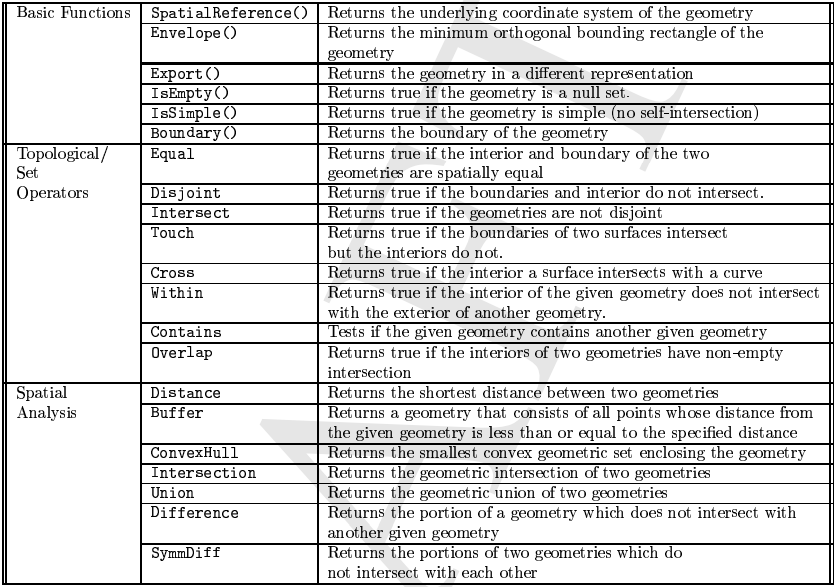
\includegraphics[height=5cm]{tablaOGIS.png}
	\end{center}
\end{frame}

\begin{frame}
		\frametitle{Ejemplos de consultas espaciales}
\end{frame}
